% =====================================================================
%  Passivity-Bounded Two-Way Modal Contact in an Interactive-Rate
%  Augmented-Lagrangian Solver   --   standalone method paper (DRAFT)
%
%  Builds with:  latexmk -pdf main.tex   (pdflatex -> bibtex -> pdflatex x2)
%
%  FORMAT: MIG (ACM SIGGRAPH conf.) = acmart sigconf. Per the MIG CFP the
%  review copy uses  \documentclass[sigconf,screen,review,anonymous]{acmart}
%  (double-blind, line numbers). Long papers: <= 10 pages EXCLUDING refs.
%  Camera-ready later drops `review,anonymous` and adds rights info.
%
%  CLAIM DISCIPLINE: see ../docs/novelty_positioning.md (do/don't list) and
%  CLAUDE.md 14 ("claims to avoid"). Do NOT claim "first two-way".
%  REAL-TIME DISCIPLINE: the validated CPU path measures 17-34 Hz (X5) --
%  say "interactive rates"; the device path is future validation work (G3).
%
%  REPOSITIONING (2026-07-13, EXECUTED): this is a STANDALONE method paper.
%  Coevoet et al. 2020 is motivation + the one-way baseline, NOT the base
%  we extend. Source-wide policy (applies to all new text):
%   - the acronym "DCR" never appears; cite \citet{coevoet2020distant},
%     or say "the one-way (forced-IIR) injection baseline";
%   - no "builds on / generalizes / base method / departure from" voice;
%   - scenes are described by what they test; layout provenance is one
%     clause, never the lead;
%   - method equations cite the standard sources (FFRF/modal analysis),
%     with Coevoet et al. as an instance, not "DCR Eq. N";
%   - "distant response" only when describing THEIR method; otherwise
%     "far-field/spatial response", "transmitted vibration".
%  The Zheng-James transcription honesty and all numbers are unchanged.
% =====================================================================
\PassOptionsToPackage{dvipsnames,table}{xcolor}
\documentclass[sigconf,screen,review,anonymous]{acmart}
% Camera-ready: \documentclass[sigconf,screen]{acmart} + rights commands.

% ---- ACM/MIG metadata (placeholders until the MIG'26 rights email) ----
\setcopyright{none}
\acmConference[MIG '26]{The 19th ACM SIGGRAPH Conference on Motion,
  Interaction and Games}{December 11--13, 2026}{Charleston, SC, USA}
\acmBooktitle{The 19th ACM SIGGRAPH Conference on Motion, Interaction and
  Games (MIG '26), December 11--13, 2026, Charleston, SC, USA}
%\acmSubmissionID{###}   % <- EasyChair paper ID once assigned
\acmDOI{}
\acmISBN{}

% ---- packages (acmart already loads: amsmath, graphicx, booktabs,
%      hyperref, natbib [numeric], xcolor, libertine/newtxmath fonts;
%      do NOT load geometry/times/amssymb -- they clash with the class) ----
\usepackage{pifont}
\graphicspath{{figures/}}

% absorb the last few sub-line-width overfulls (only stretches lines that would
% otherwise overflow; leaves well-set lines untouched)
\setlength{\emergencystretch}{8pt}

% pack float pages tighter — content sits at the 10-page MIG cap
\renewcommand{\topfraction}{0.95}
\renewcommand{\bottomfraction}{0.6}
\renewcommand{\textfraction}{0.05}
\renewcommand{\floatpagefraction}{0.85}
\renewcommand{\dbltopfraction}{0.95}
\renewcommand{\dblfloatpagefraction}{0.85}

% ---- draft helpers (delete for camera-ready) ----
\newcommand{\todo}[1]{\textcolor{red}{\textbf{[TODO: #1]}}}
\newcommand{\note}[1]{\textcolor{Plum}{\textit{(#1)}}}
\newcommand{\yes}{\textcolor{ForestGreen}{\ding{51}}}
\newcommand{\no}{\textcolor{BrickRed}{\ding{55}}}
\newcommand{\pmark}{\textcolor{orange}{$\sim$}}   % partial / genre-only
\newcommand{\pend}{\textcolor{gray}{$\circ$}}      % planned / pending measurement
\newcommand{\na}{\textcolor{gray}{---}}            % not applicable
\newcommand{\q}[1]{{\scriptsize\,#1}}              % compact in-cell qualifier

% ---- notation ----
\newcommand{\amp}{\mathbf{a}}          % modal amplitude vector (the code's q)
\newcommand{\nvec}{\hat{\mathbf{n}}}
\newcommand{\Phimat}{\boldsymbol{\Phi}}
\newcommand{\Ghat}{\hat{\mathbf{G}}}
\newcommand{\dEmod}{\Delta E_{\mathrm{modal}}}
\newcommand{\dErig}{\Delta E_{\mathrm{rigid}}}

% DEVIATION from earlier draft title: "Real-Time" -> "Interactive-Rate"
% until the device path is passivity-validated (experiment plan G3).
\title{Passivity-Bounded Two-Way Modal Contact in an Interactive-Rate
       Augmented-Lagrangian Solver}

\author{Nan Li}
\orcid{0000-0000-0000-0000} % TODO: real ORCID (required by ACM at camera-ready)
\affiliation{%
  \institution{University of Southern California}
  \city{Los Angeles}\state{CA}\country{USA}}
\email{nli62220@usc.edu}
% \note{co-authors / advisor TBD -- add \author blocks before submission}

\begin{document}

% acmart requires abstract, CCS, and keywords BEFORE \maketitle.
\begin{abstract}
We bring \emph{two-way} rigid--modal contact coupling into the fixed-iteration
position-based / augmented-Lagrangian rigid-body solvers that interactive
applications already run (XPBD, AVBD). Each body's linear vibration modes are
carried as a handful of compliant-constraint degrees of freedom: a single
shared unilateral contact multiplier both excites the modes of the bodies in
contact and reacts on their rigid frames through equal-and-opposite Jacobian
blocks, and vibration propagates through a body--body contact network. The
constraint law itself is classical --- linearized, our position-level contact
row recovers the velocity-level rigid--modal contact constraint of Zheng and
James --- but its direct transcription into a solver running at a fixed, low
iteration budget is not energy-safe: the under-converged stiff modal block
injects spurious energy, or diverges outright. The contributions are the
solver couplings that keep that block stable at a fixed budget, and an
enforced passivity inequality $\dEmod \le \eta\,\dErig$ on the
contact$\to$modal transfer, maintained cumulatively across every substep of
every run, which together make two-way modal contact usable at interactive
rates. We validate deformation amplitude, frequency, and spatial profile
against a full-FEM ground truth; a GPU-resident co-solved path reaches
$120$~Hz real-time rates and sustains $512$ bodies while a per-run ledger
verifies the same bound, and the bounded excitation stream drives a standard
modal impact-sound render.
\end{abstract}


\begin{CCSXML}
<ccs2012>
<concept>
<concept_id>10010147.10010371.10010352.10010379</concept_id>
<concept_desc>Computing methodologies~Physical simulation</concept_desc>
<concept_significance>500</concept_significance>
</concept>
</ccs2012>
\end{CCSXML}
\ccsdesc[500]{Computing methodologies~Physical simulation}

\keywords{rigid-body dynamics, modal reduction, contact, passivity,
  augmented Lagrangian, XPBD}

% TODO(teaser): \begin{teaserfigure} with a render strip once W5 lands.
%   Panels sell the standalone story --- candidate strip: stack ring
%   through contacts | native-vs-FEM overlay | clamp-off blow-up. No
%   baseline-layout branding in the caption. (E-R1 topple control did NOT
%   pan out as a panel: knife-edge, platform-FP-sensitive — see 40_results.)

\maketitle

\section{Introduction}
\label{sec:intro}

\paragraph*{Motivation.} Rigid-body simulators are fast because they discard
deformation, but real objects ring, chatter, and transmit vibration through their
contacts. Modal reduction restores that behaviour cheaply by tracking a handful of
vibration modes per body. The open question is how tightly the modal layer is
\emph{coupled} to contact: whether contact merely \emph{reads} rigid motion and adds
a cosmetic vibration (one-way), or whether the vibration \emph{reacts} back on the
bodies and on their neighbours through the same contact (two-way).

\paragraph*{The gap.} \citet{zheng2011} resolve modal vibration inside both the
collision and frictional-contact stages, producing genuinely coupled motions --- but
at large computational cost, in an offline velocity-level solver.
\citet{coevoet2020distant} (DCR) make this affordable for real time by dropping the
back-reaction: they inject a distant collision response as a one-way velocity change
and the simulation ``remains rigid.'' Neither offers a guarantee on the \emph{energy}
the contact injects into the modes.

\paragraph*{This paper.} We embed the vibration modes as native compliant constraints
inside an interactive-rate augmented-Lagrangian / position-based rigid solver
(XPBD~\citep{macklin2016xpbd}, VBD/AVBD~\citep{chen2024vbd,giles2025avbd}). One
unilateral contact multiplier excites the modes and reacts on the bodies within the
same solver iteration (\S\ref{sec:method}). This fixed-budget regime \emph{creates} a
failure mode the convergent offline solver never had: an under-converged local solve
can inject spurious energy into the stiff modal block. Our remedy is an enforced
passivity bound $\dEmod \le \eta\,\dErig$ on the contact$\to$modal transfer ---
maintained cumulatively every substep by an exact energy projection
(\S\ref{sec:method:passivity}) --- which makes the
coupling usable at a fixed low iteration budget. We generalize the invariant across a
body--body modal contact network and validate against a full-FEM ground truth
(\S\ref{sec:results}).

\paragraph*{Contributions.}
\begin{itemize}
  \item A cumulative \textbf{directional energy budget} on the transfer from
        contact into the modes, funded by measured rigid contact loss and
        enforced by an exact modal-state projection
        (\S\ref{sec:method:passivity}). Prior energy-stable contact constrains
        the \emph{system} --- non-increase, whole-system passivity, or
        conservation projection (\S\ref{sec:related}) --- not the one-sided,
        source-referenced transfer.
  \item Vibration modes as \textbf{first-class compliant-constraint DOFs}
        sharing one unilateral contact multiplier with the rigid solve of a
        fixed-budget augmented-Lagrangian host --- prior interactive modal
        contact used LP constraints or penalties (\S\ref{sec:related}); the
        shared fixed-budget AL row, and what its truncation does to energy,
        is the new embedding.
  \item That bound \textbf{generalized across a body--body modal contact
        network} --- stacked bodies ring through their shared contacts.
  \item Validation against a full-FEM ground truth and a contact-force audit
        (\S\ref{sec:results}).
\end{itemize}

\section{Related Work}
\label{sec:related}

\todo{Expand each paragraph; this is a seeded map from the prior-art audit
(\texttt{docs/novelty\_positioning.md}).}

\paragraph*{Modal sound and contact.} \citet{zheng2011} carry modal amplitudes as
generalized coordinates driven two-way by a shared contact multiplier, resolving
vibration in both the collision and friction stages; the coupling is
momentum-consistent by construction but solved offline as a global staggered LCP/QP
at large cost. \citet{james2002dyrt} render one-way real-time modal response
(display-only, no back-reaction). DCR~\citep{coevoet2020distant} is the real-time,
one-way distant response this project builds on and generalizes.

\paragraph*{Reduced bodies as contact DOFs.} Affine Body
Dynamics~\citep{lan2022abd} makes a $9$-DOF affine subspace a native contact DOF
inside IPC; it captures uniform stretch/shear but not the bending/plate modes that
carry the distant response, and carries no energy-transfer bound.
\citet{sheth2015} give fully momentum-conserving reduced deformable contact ---
two-way and conserving \emph{momentum}, but not bounding \emph{energy}. Classical
floating-frame / component-mode multibody (\citealp{shabana_multibody};
energy--momentum integrators, \citealp{betsch2007}) couple modal reduction with
contact but \emph{conserve} energy rather than \emph{cap} the directional transfer.

\paragraph*{Passivity.} Port-Hamiltonian flexible multibody
dynamics~\citep{brugnoli2021} and time-domain passivity control in
haptics~\citep{hannaford2002} give the passivity-inequality \emph{genre}, but not a
contact$\to$modal transfer budget of the form $\dEmod\le\eta\,\dErig$.

\paragraph*{Real-time augmented-Lagrangian solvers.}
XPBD~\citep{macklin2016xpbd} and VBD/AVBD~\citep{chen2024vbd,giles2025avbd} host
rigid and soft contact at a fixed low iteration budget on the GPU, but carry no modal
DOFs --- the slot this paper fills.

\paragraph*{Positioning.} Table~\ref{tab:positioning} places the method: two-way
\emph{and} real-time \emph{and} passivity-bounded is the cell neither Zheng and James
(offline) nor DCR (one-way) occupy.

\begin{table}[t]\centering
\caption{Where the method sits. \note{Do not claim the first two columns as novel ---
they are the mechanism Zheng and James already had.}}
\label{tab:positioning}
\begin{tabular}{lccc}
\toprule
 & two-way & real-time & passivity bound \\
\midrule
Zheng \& James 2011 & \yes & \no & \no \\
DCR (Coevoet 2020)  & \no  & \yes & \no \\
\textbf{This paper} & \yes & \yes & \yes \\
\bottomrule
\end{tabular}
\end{table}

\section{Method}
\label{sec:method}

\todo{Expand derivations; cite the paper/foundation equation numbers per CLAUDE.md.}

\subsection{Modes as native contact constraints}
\label{sec:method:constraint}
Each body carries mass-normalized linear modes $\Phimat$ with amplitudes $\amp$ (the
code's $q$). A contact with unit normal $\nvec$ acts on the \emph{deformed} contact
point of both participants, so the unilateral gap becomes
\begin{equation}
  C \;=\; C_{\mathrm{rigid}} \;+\; \big(\Ghat_A\!\cdot\amp_A - \Ghat_B\!\cdot\amp_B\big),
  \qquad \Ghat_X = \nvec^{\!\top} R_X\, \Phimat_X ,
  \label{eq:gap}
\end{equation}
where $R_X$ is body $X$'s rotation. Writing $z=(v,\omega)$ for a body's rigid
velocity DOFs, the full gradient of one contact row (lever arms $r_A,r_B$ from each
COM) is the ordinary rigid Jacobian extended by one modal column block per
participant:
\begin{equation}
  \frac{\partial C}{\partial z_A} = \begin{bmatrix}\nvec\\ r_A\!\times\!\nvec\end{bmatrix}\!,
  \;\;
  \frac{\partial C}{\partial z_B} = -\begin{bmatrix}\nvec\\ r_B\!\times\!\nvec\end{bmatrix}\!,
  \;\;
  \frac{\partial C}{\partial \amp_A} = +\Ghat_A,
  \;\;
  \frac{\partial C}{\partial \amp_B} = -\Ghat_B.
  \label{eq:grad}
\end{equation}
A single contact multiplier $f\ge 0$ then (i)
pushes the rigid bodies apart and (ii) drives each participant's modes by
$+\Ghat_A f$ on $A$ and $-\Ghat_B f$ on $B$. Newton's third law is built in, so the
coupling is two-way and momentum-consistent by construction --- not a post-solve
kick. The support contact (body$\leftrightarrow$ground) is the \emph{same} row type
with the ground as degenerate participant: the surface is
$y_{\mathrm{rest}}+U_y^{\!\top}q_s$, so $\partial C/\partial q_s=-U_y$ with $U_y$
the support mode shapes' vertical components at the contact's footprint. That is
the whole generalization --- every body with modes participates, including stacked
bodies that only ever touch another body. Mass-normalized modes give
$M_q=I$, $K_q=\operatorname{diag}(\omega_j^2)$, $D_q=\alpha_0 I+\alpha_1 K_q$
(Rayleigh; DCR Eq.~7), so no reduced inverse is ever formed.
\note{This unified $(z,Q)$ row is documented in \texttt{two\_band\_coupling.html} and
\texttt{docs/sheldon\_report/README.md}.}

\subsection{Solving the stiff modal block in a local iteration}
\label{sec:method:solve}
A global QP absorbs a stiff modal DOF ($K_q\!\sim\!10^{11}$) implicitly for free; a
fixed low-iteration \emph{local} solver makes that stiff, dense modal block diverge
under naive Gauss--Seidel. Making it stable \emph{and} two-way there is the
algorithmic content of this section, and the reason the passivity bound of
\S\ref{sec:method:passivity} is needed. We embed the row of Eq.~\ref{eq:grad} in
both solver families.

\paragraph*{AVBD (augmented Lagrangian).} Each contact carries a penalty-plus-
multiplier force $f=\max(0,\rho\,C+\lambda)$; body blocks solve their usual
$6\times6$ systems with Hessian $M/h^2+\sum\rho\,J^{\!\top}J$. The modal amplitudes
are chased in a separate \emph{engaged-gated block Gauss--Seidel} pass after each
body sweep: only rows with an active multiplier contribute, and the modal block is
solved implicitly (backward Euler) as
\begin{equation}
  \Big(\tfrac{1}{h^2}M_q+\tfrac{1}{h}D_q+K_q\Big)\,\Delta\amp
  \;=\; \textstyle\sum_{\mathrm{engaged}}\Ghat^{\!\top} f
        \;-\; K_q\,\amp \;-\; \tfrac{1}{h}D_q\,(\amp-\amp^{\mathrm{prev}}),
  \qquad
  \amp \leftarrow \amp + \omega_r\,\Delta\amp,
  \label{eq:qblock}
\end{equation}
with under-relaxation $\omega_r$ (\texttt{modal\_relax}, $0.7$ in production; the
diagonal $M_q,K_q,D_q$ make the solve $r$ independent scalar updates). The
alternative --- condensing the modal columns into the contact solve by a cross-term
Schur complement --- was measured to inject energy because the eliminated
$\Delta z$ is never back-substituted at a truncated iteration count; the gated
block-GS with explicit $\Delta\amp$ is what remains stable at $8\!-\!16$
iterations.

\paragraph*{XPBD (compliant position-level).} The same row becomes a compliant
constraint with $\tilde\alpha=\alpha/h^2$ and damping $\gamma$; the generalized
inverse mass simply gains the modal terms of Eq.~\ref{eq:grad},
\begin{equation}
  w \;=\; J M^{-1} J^{\!\top}
        \;+\; \Ghat_A M_{q,A}^{-1}\Ghat_A^{\!\top}
        \;+\; \Ghat_B M_{q,B}^{-1}\Ghat_B^{\!\top},
  \qquad
  \Delta\lambda \;=\; \frac{-C-\tilde\alpha\lambda-\gamma\,\dot C}
                            {(1+\gamma)\,w+\tilde\alpha},
  \label{eq:xpbd}
\end{equation}
after which positions and amplitudes update along the gradient,
$\Delta\amp_A=+M_{q,A}^{-1}\Ghat_A^{\!\top}\Delta\lambda$ (mass-normalized:
$M_q^{-1}=I$), scaled by the same under-relaxation. The modal internal dynamics
enter as per-mode compliant rows with $\alpha_j=1/\omega_j^2$. The formulation
difference matters: the AVBD chase tolerates $\omega_r=0.7$, while the XPBD
Gauss--Seidel has a measured ceiling of $\omega_r=0.25$ on the stiff scenes
($0.5$--$0.6$ ejects bodies, ${\ge}0.65$ NaN) --- one direct motivation for the
formulation-level passivity analysis below.

\subsection{The passivity bound}
\label{sec:method:passivity}
Because the local solve under-converges, the contact can inject energy into the
modes. We cap the per-step contact$\to$modal transfer by
\begin{equation}
  \dEmod \;\le\; \eta\,\dErig , \qquad \eta\in[0,1],
  \label{eq:passivity}
\end{equation}
enforced globally across all contacts each rigid step (foundation \S15). A passive
scaling coefficient $\alpha\in[0,1]$ solves the per-step quadratic
$\dEmod(\alpha)=\alpha b + \tfrac12\alpha^2 a \le E_{\max}$ (foundation \S6),
so the injected energy never exceeds the fraction $\eta$ of the rigid kinetic energy
lost during contact resolution.
\note{DEVIATION from DCR Eq.~10 (forced IIR): the injection is a velocity-level kick
to $\dot q$ funded by rigid kinetic-energy loss, not a forced response --- see
CLAUDE.md and the foundation \S15.}

\section{Results}
\label{sec:results}

We evaluate on the scenes of Table~\ref{tab:scenes}: DCR's own road, dinner, and
ledge figure layouts --- re-simulated with the two-way modal-constraint coupling in
place of DCR's one-way injection --- plus two modal-network stress scenes
(a box--box cube stack and a two-body full-FEM reference). Reusing DCR's layouts is
deliberate: it lets us show, on the same scenes, the back-reaction DCR cannot
produce (a distant body moved \emph{by} another body's ring through their shared
contact).

Table~\ref{tab:matrix} is the validation matrix. Each row is a metric scored against
a named reference baseline; each column is a scene. \yes\ marks a measured result
(number in the cell, subsection cited); \pend\ marks a measurement planned against
the full-FEM ground truth currently being wired; \na\ marks not-applicable. The
matrix doubles as the experiment tracker --- the honest current state is that the
contact-force ledger, the two-way network discriminator, and the passivity ablation
are measured, while the cross-scene FEM-accuracy and runtime rows are pending.

\paragraph*{Baselines (the reference axis).} Metrics are scored against:
\textbf{F} --- a full-FEM (unreduced) solve of the same mesh, the accuracy ground
truth \note{(consider IPC~\citep{lan2022abd}-grade contact for the reference; a
penalty/linear-implicit FEM under-resolves stiff contact)};
\textbf{D} --- DCR one-way (rigid $+$ separate IIR, no back-reaction), the base
method;
\textbf{R} --- rigid-only (modes off), the cost floor and the two-way null;
\textbf{A} --- the analytic static ledger ($\sum\lambda = mg$);
and the two internal toggles \textbf{off/on} (passivity clamp; modal network) that
isolate the two claims that are ours alone.

\begin{table}[t]\centering\footnotesize
\setlength{\tabcolsep}{4pt}
\caption{Evaluation scenes. Rows 1--3 are DCR's own figure layouts re-simulated with
two-way coupling; rows 4--5 are modal-network stress scenes. $n_g/n_\ell$ =
global/local reduced modes per body; body counts for dinner/ledge are the measured
X5 scene sizes. \todo{fill the road body count from the built truck scene.}}
\label{tab:scenes}
\begin{tabular}{llccl}
\toprule
scene & source & bodies & $n_g/n_\ell$ & what it tests \\
\midrule
Road (crate/cones)    & DCR road  & \todo{N}        & 12/16 & distant response, large slab \\
Dinner table          & DCR Fig.1 & 17              & 10/14 & distant place-settings \\
Ledge (boulder)       & DCR ledge & 5               & 12/16 & strong-coupling topple \\
Cargo network (stack) & ours      & 6              & 8/1   & two-way, box--box network \\
FEM cargo             & ours      & 2              & 8/1   & full-FEM accuracy reference \\
\bottomrule
\end{tabular}
\end{table}

\begin{table}[t]\centering\footnotesize
\setlength{\tabcolsep}{3.5pt}
\caption{Validation matrix: metric $\times$ scene, each scored against a reference
baseline (col.\ \textbf{ref}, key above). \yes\ measured (number cited); \pend\
planned vs.\ full-FEM; \na\ not applicable. The two rows no prior method can pass ---
the passivity bound and the two-way discriminator --- are already measured on the
stack; the cross-scene FEM-accuracy rows are the pending work.}
\label{tab:matrix}
\begin{tabular}{llccccc}
\toprule
metric & ref & Road & Dinner & Ledge & Stack & FEM \\
\midrule
Modal displ.\ $L_2$ error          & F      & \pend & \pend & \pend & \pend & \pend\q{.56$\to$1.02} \\
Distant-response fidelity          & F,D    & \pend & \pend & \pend & \na   & \na \\
Contact-force ledger               & A      & \pend & \na   & \pend & \yes\q{.06--1.9\%} & \na \\
Passivity $\dEmod\!\le\!\eta\dErig$ & bound  & \pend & \pend & \pend & \yes  & \pend \\
Momentum drift (lin/ang)           & $0$    & \pend & \pend & \pend & \pend & \pend \\
Two-way ring $|\amp|$              & off/on & \pend & \pend & \pend & \yes\q{1.1e{-}5/0} & \na \\
Runtime (ms/step, RT$\times$)      & R,D    & \pend & \pend & \pend & \pend & \pend \\
Passivity ablation (blow-up)       & off/on & \na   & \na   & \na   & \yes\q{X1} & \na \\
\bottomrule
\end{tabular}
\end{table}

\subsection{Contact forces balance a cube stack}
\label{sec:results:ledger}
\note{Numbers below are read straight off the solver's contact multipliers; see
\texttt{docs/sheldon\_report/} and its reproduce script --- analysis only, no solver
code changed.} A modal slab carries a plain resting control cube and a 3-high zig-zag
stack (base/mid/upper); each cube carries its own reduced modes. Reading the
multipliers (Table~\ref{tab:ledger}), each joint carries exactly the weight above it,
with no per-joint tuning --- the shared multiplier balances the tower on its own.

\begin{table}[t]\centering
\caption{Static contact ledger (settled), $m g = 5.886$~N.}
\label{tab:ledger}
\begin{tabular}{lccc}
\toprule
joint & measured & expected & error \\
\midrule
resting cube $\to$ slab                & 5.889~N & $mg$  & 0.06\% \\
base cube $\to$ slab                   & 17.99~N & $3mg$ & 1.9\%  \\
base $\leftrightarrow$ mid (box--box)  & 11.93~N & $2mg$ & 1.4\%  \\
mid $\leftrightarrow$ upper (box--box) & 5.82~N  & $mg$  & 1.1\%  \\
\bottomrule
\end{tabular}
\end{table}

\begin{figure}[t]\centering
  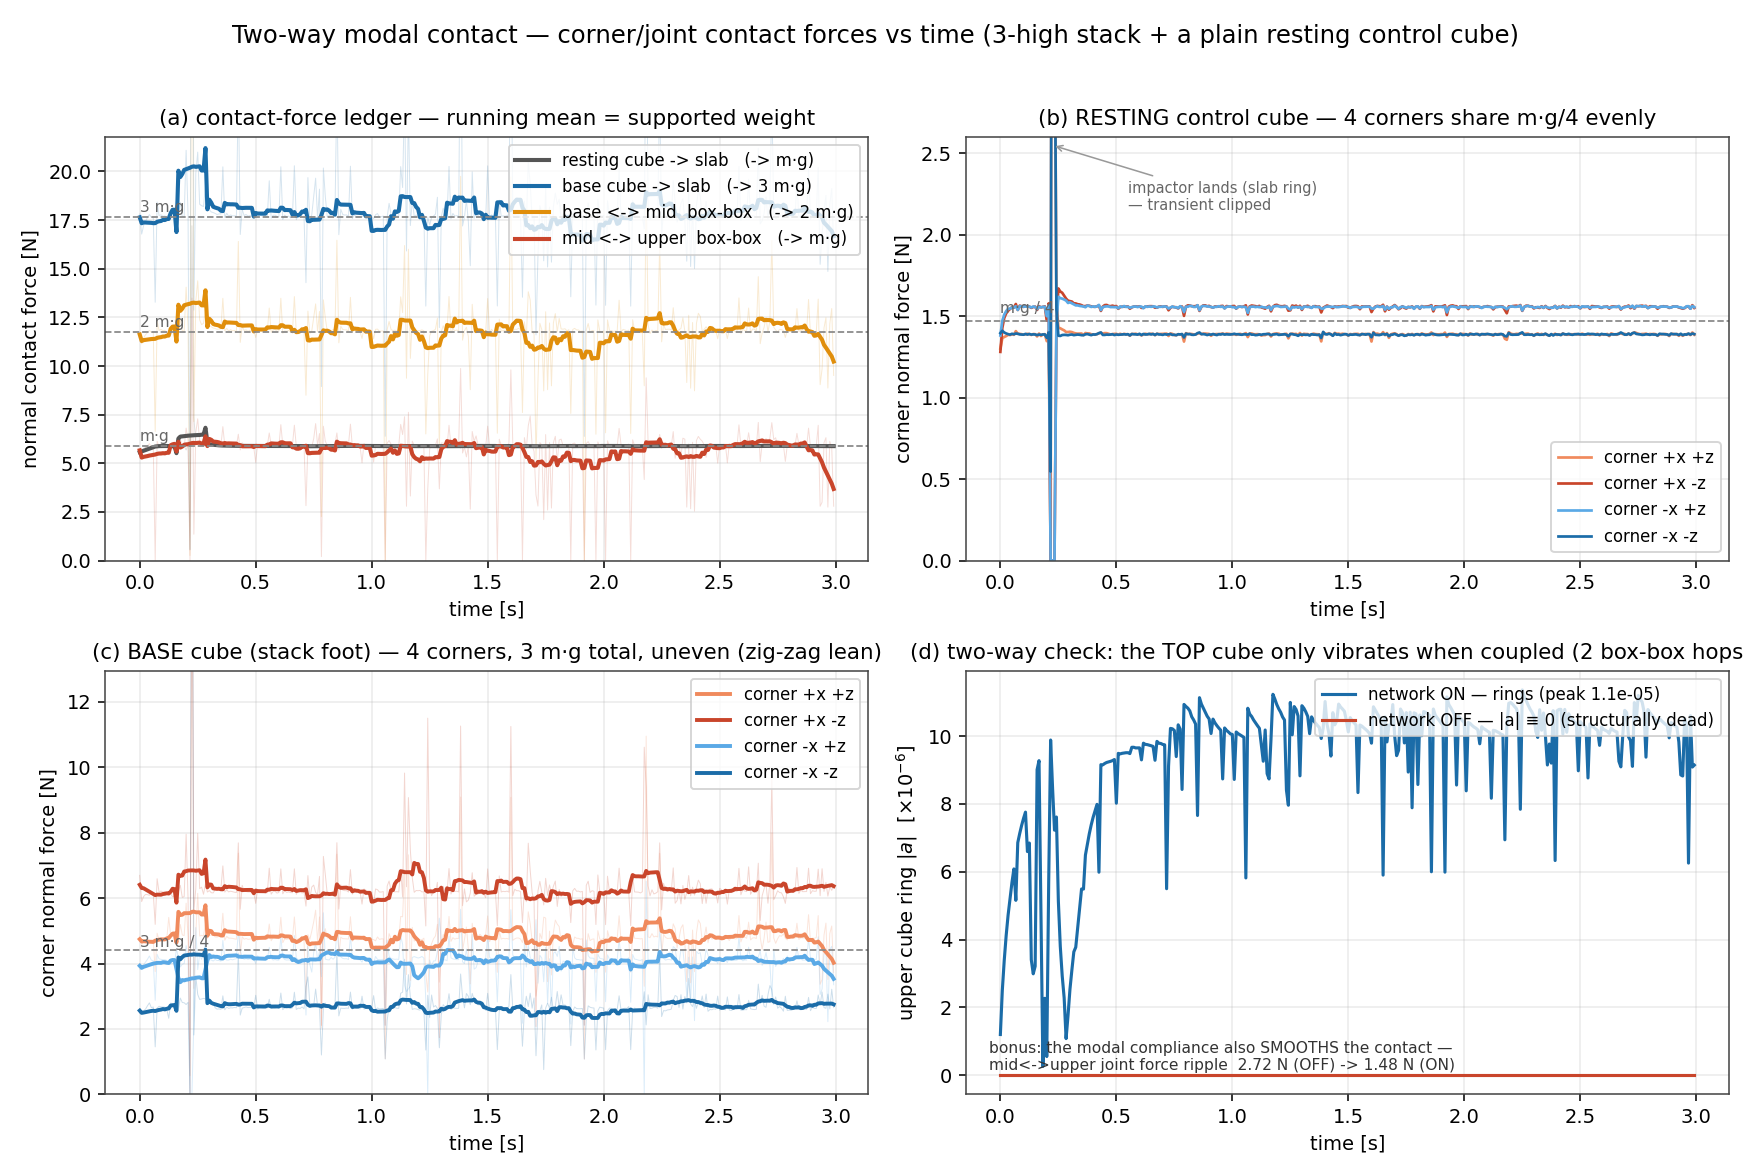
\includegraphics[width=\linewidth]{contact_forces.png}
  \caption{Per-corner / per-joint normal contact force vs.\ time. The plain resting
  cube shares $mg$ evenly across its 4 corners; the stack foot carries $3mg$ split
  \emph{unevenly} where the tower leans; the top cube --- two box--box hops from the
  slab --- rings only when the network is on ($|\amp|\!\equiv\!0$ off), the two-way
  discriminator.}
  \label{fig:forces}
\end{figure}

\subsection{Two-way through the network}
\label{sec:results:network}
The \texttt{upper} cube touches only \texttt{mid}; with the modal contact network on
it rings ($|\amp|$ peak $\approx 1.1\times10^{-5}$), off it is identically zero. The
vibration reaching it arrives only through the shared contacts. The modal compliance
also \emph{smooths} the box--box force (joint-force ripple $\pm2.72$~N off
$\to \pm1.48$~N on, mean unchanged at $mg$).

\subsection{Full-FEM ground truth}
\label{sec:results:fem}
\todo{Report the C3 convergence: reduced-vs-full-FEM ratio $0.56 \to 1.02$ as
$h\to0$ (X-suite).}

\subsection{The passivity bound bites when it must}
\label{sec:results:passivity}
\todo{Report X1: clamp off injects up to ${\sim}1.2\times10^{5}\times$; clamp on is
passive; inert at high iteration budget, active at the low budget ($8\times2$).}

\section{Conclusion and Limitations}
\label{sec:conclusion}

\todo{Write once results are frozen.}

We embedded vibration modes as first-class compliant-constraint DOFs in a real-time
augmented-Lagrangian rigid solver, driven two-way by a shared unilateral contact
multiplier, and made the coupling stable at a fixed low iteration budget with an
enforced passivity bound $\dEmod\le\eta\,\dErig$.

\paragraph*{Limitations \note{(binding: foundation \S14 ``claims to avoid'').}}
\begin{itemize}
  \item The two-way coupling \emph{mechanism} is not new
        (\citealp{zheng2011}); the contribution is its real-time-AL embedding and the
        passivity bound.
  \item The bound applies to the modal-path injection only; the
        spatial-attenuation path is empirical and not energy-budgeted.
  \item Small-displacement regime only: support contact rows sample the modal
        basis at each contact's rest footprint with a fixed vertical normal
        (DCR instead re-maps contacts barycentrically every step), and the
        linearized modes carry no geometric stiffening --- valid at the
        mm-scale responses shown, not for span-scale deflections.
  \item The rigid step band-limits the impact transient: dish-launch
        amplitudes run well under the full-FEM reference at $h=1/120$ and
        recover monotonically with the step ($16\times$ over an $8\times$
        ladder, \S\ref{sec:results:fem}) without reaching it --- though the
        reference launch observable is itself contact-model-limited, so the
        residual is an upper bound on the true deficit. DCR's sub-stepped
        IIR kick re-amplifies that transient at the cost of passivity
        (\S\ref{sec:results:restitution}).
  \item Native contact restitution is $e{=}0$: the sweep of
        \S\ref{sec:results:restitution} shows the energy ratio stays bounded at
        every $\varepsilon_r$ by construction, but a matched-restitution
        comparison against DCR needs a Newton restitution term in the native
        contact --- future work.
  \item Scene breadth: all road-scene accuracy rows are pending (qualitative
        only), and the affine (ABD) basis showed a slow secular buildup and
        would need the same governor before any stability claim.
\end{itemize}

\paragraph*{Future work.} A swappable affine (ABD) cargo basis for cheap, robust
contact, energy-governed the same way; \todo{$\ldots$}


\bibliographystyle{ACM-Reference-Format}
\bibliography{references}

\end{document}
